%!TEX ROOT=main.tex

This chapter will walk the reader through the various options that were considered and final choices that were made during the concept and initial design stages of this project.

\section{Separation of concerns}
As was discussed in the Introduction \ref{chapter:introduction}, the main goal of this work is the soil moisture sensor hardware with the accompanying firmware and a proof-of-concept application.

With that being said, one can easily discern separate sub-tasks within this broader goal - mainly the fact, that the communication aspect can be separated from the sensor itself (see Figure \ref{fig:device-split}) a practice commonly seen in the industry.

\begin{figure}
    \includesvg[width=\textwidth]{fig/3_device-split.drawio.svg}
    \caption{\label{fig:device-split} Logical high level building blocks of most modern sensors}
\end{figure}

Separating these two concerns not only logically, but also on the hardware level, will bring many advantages - future sensor implementations can be made with only effort being put into the sensor itself; the wireless part and most of the testing and regulation overhead can be solved once, not repeated for every sensor type; once a sensor compatible with the interface exists, it can be made compatible with future versions of the interface - to list a few.

While this work is mainly concerned with the soil moisture sensing application, having a LoRa compatible unit, which is capable of OTA updates and has enough processing power to handle most sensing and simple control task, while being power-efficient enough to be battery powered, is an interesting sub-goal of this work.

The following sections will go through the process of finding requirements for such hardware and explain the compromises made.

\section{Module requirements}
\subsection{\label{section:application-case-studies} Application case-studies}
In order to find the optimal boundary between the sensor implementation part and the Interface and Processing part, as defined in Figure \ref{fig:device-split}, it is useful to look at the possible applications of the proposed module.

\subsubsection{Indoor environment sensor array}
Let us consider this basic, typical, use-case for such a communication module. This application can implement the following sensors
\begin{itemize}
    \item thermometer
    \item hygrometer (relative humidity sensor)
    \item human presence detector
    \item air quality sensor (CO$^2$e, smoke, ...)
    \item light sensor
\end{itemize}
we can omit some of the listed sensors in the actual application, but the module should be able to support the full configuration without any kind of co-processor. Main limiting factor will probably be the number of communication peripherals a General Purpose Input Output pins.

Thermometer is usually an integral part of any hygrometer measuring relative humidity \cite{webster_humidity_1998}, that is also suitable for this application. These sensors are frequently found in fully integrated solutions with a digital interface of some sort, usually I2C \cite{bosch_sensortec_gmbh_bst-bme280-ds002pdf_2024}. The same is true for any modern light sensor, which will also be able to measure intensities of different wavelengths of light \cite{stmicroelectronics_ambient_2024}, \cite{texas_instruments_inc_light_2024}. Thus more than half of the sensors listed only require a single I2C port to control them comfortably.

Traditionally, PIR sensors are used to detect motion, thus presence of humans in the vicinity of the sensor, but this might not work reliably for indoor applications. Thus, nowadays, the use of radar-based systems \cite{ag_presence_2024} or IR ranging sensors \cite{stmicroelectronics_human_2024} are a lot more prevalent for human presence detectors. Such a sensor might expose a digital interface, such as I2C or SPI, or simply output an analog signal, which can be sampled using an ADC.

Other environmental sensors, such as air quality sensors, also implement similar interfaces - I2C or SPI or an analog output. Notably these sensors usually exhibit relatively high power draw ($>100~\mathrm{mW}$) and slowest startup times of all the other sensors of this application (orders of 10s of seconds to minutes) \cite{amphenol_inc_mics-vz-89te_2024}, so they are not suitable for battery-powered applications.

On the note of power draw, this application may wish to be battery powered or remain mains powered, this will affect the capabilities and the end use-case. 

When running on battery, the active on-time is limited to periodic sampling of the environment a handful times per hour. Being able to power down all sensors can prove useful in this application to greatly improve the battery life. On the other hand, if the application aims at fast reaction times, switching on the lights when presence detected for example, and the inclusion of all the sensors listed, it will need to be mains powered to be practical.

\subsubsection{Light dimmer}
For this application only a timer peripheral capable of generating PWM of sufficient frequency and resolution on a handful of channels is needed. Such peripheral exists on most modern microcontrollers.

If local control is also required, a rotary encoder for example, which can be sampled using a digital input interrupt or a dedicated peripheral designed to handle encoders.

\subsubsection{Soil moisture sensor}
The defining features of this application are outdoor use, battery power with the possibility of including a solar panel for zero-maintenance operation, long range and low dynamic duty-cycle.

solární článek a nabíjecí obvod by se integroval spolu s obvody pro měření vlhkosti na PCB samotného senzoru. pro bateriové aplikace jsou tudíž ideální LiFePO4, které mají pracovní rozsah 2.5-3.6V, což je v pracovním rozsahu STM32 a většiny dalších 3V3 komponent

\subsubsection{Gateway}
The module should be versatile enough to be also able to act as a communication interface for a host computer to connect to and manage the network of sensors, though other more specialized hardware could also be used for this use-case.

\subsection{Over-the-air update support}

doplnit jakmile to bude v uvodu

\subsection{\label{section:final-requirements} Final requirements}
\begin{itemize}
    \item 2V8-3V3 nominal voltage range - the lower the minimum threshold, the better (for being able to harvest as much energy as possible from ie. a coin-cell battery)
    \item low power design - support for switchable power rails for standby modes, low duty cycle operation, low power standby of the module itself
    \item target the 865-923 MHz (EU868, US915, IN865, ...) frequency range
    \item wide temperature range for outdoor applications
    \item support for wide range of use-cases - minimize the amount of specialized hardware on the module, leave that up the implementation
    \item minimal footprint
    \item support for OTA updates - large enough internal storage
    \item integrated RF - ideally a built-in antenna or some means to connect one
    \item host communication interface
    \item low cost
\end{itemize}

\subsubsection{Existing hardware satisfying these requirements}

SeedStudio Wio-E5-LE \cite{stmicroelectronics_lora_2024, seeedstudio_wio-e5-wireless_2024} is a cost effective LoRa module integrating the STM32WLE5JC SOC.

%\begin{table}[!h]
%\begin{center}
%\caption{\label{table:existing-modules} Existing modules satisfying project requirements}
%    \begin{tabular}{|l|c|c|c|} 
%    \hline
%    Name & Col2 & Col2 & Col3 \\
%    \hline
%     & 6 & 87837 & 787 \\ 
%    \hline
%    \end{tabular}
%\end{center}
%\end{table}

\section{Module architecture and parts selection}

Solderable PCB modules are a standard way of integrating existing solutions into custom ones. Modules providing wireless connectivity in particular are very common, see Figure \ref{fig:wireless-modules}.

\begin{figure}
    \centering
    \subfloat[Omega 2S]{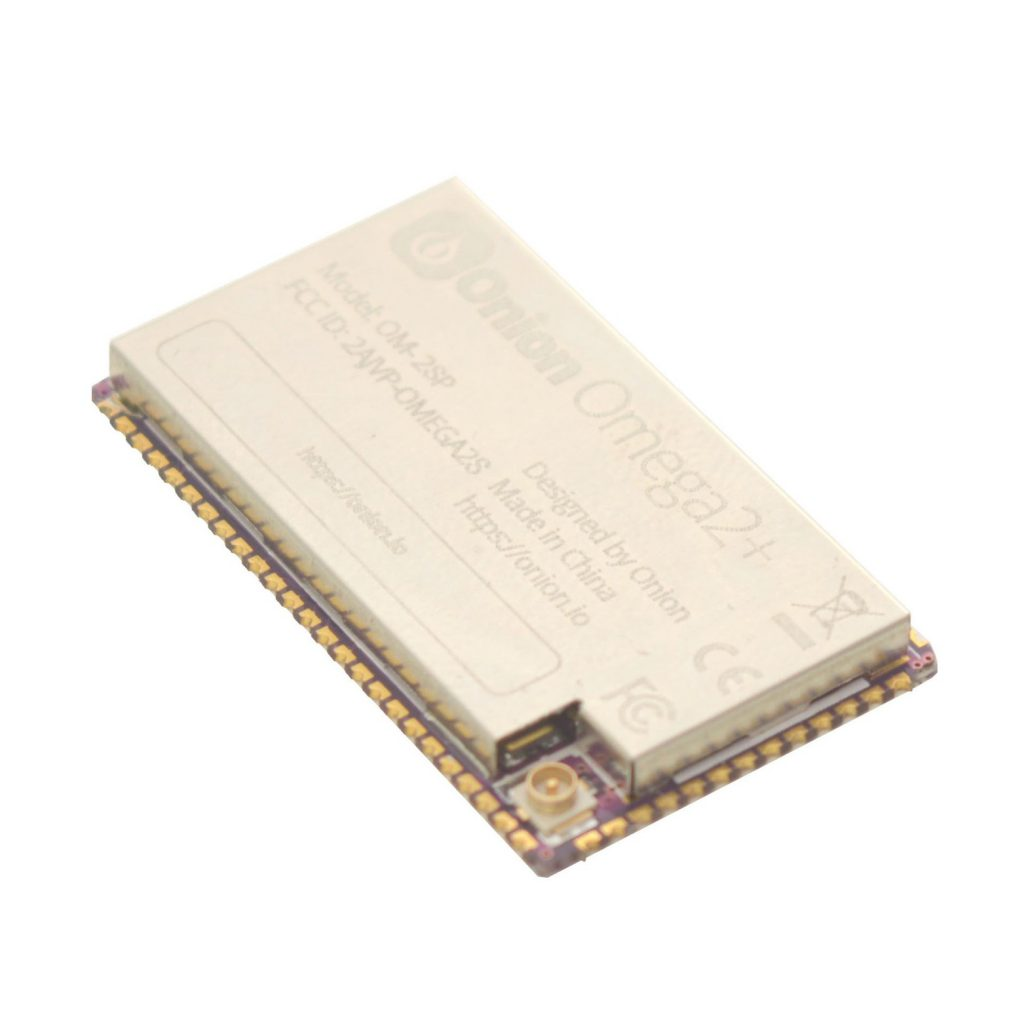
\includegraphics[width=.3\textwidth]{img/Omega2S.jpg}}
    \subfloat[RN4871]{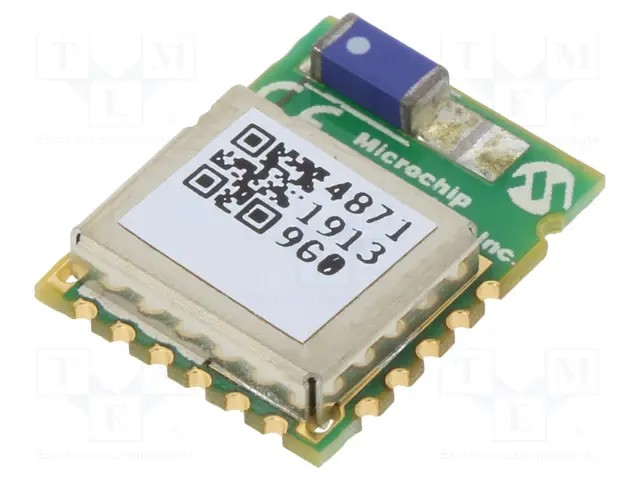
\includegraphics[width=.3\textwidth]{img/rn4871.jpg}}
    \subfloat[MAX F10s]{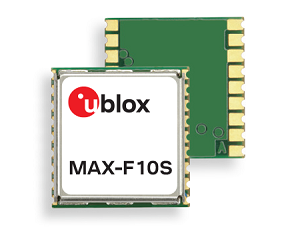
\includegraphics[width=.3\textwidth]{img/max-f10s.png}}
    \caption{\label{fig:wireless-modules} Common wireless modules}
\end{figure}
%https://onion.io/omega2s/
%https://www.microchip.com/en-us/product/rn4871
%https://www.u-blox.com/en/product/max-f10s-module

This approach allows us to separate the usually complex and more expensive multi-layer board layouts, required by modern SOCs, along with their power delivery and any other supporting circuitry, from the less complex end-application consisting of local power regulation, battery management, connectors and other mechanical features.

In order to satisfy the requirements \ref{section:final-requirements}, the module should provide means for analog and digital signal acquisition, digital communication interfaces and sufficient internal storage along with implementing the wireless connectivity.

\subsection{\label{section:mcu}Microcontroller}
Given the requirements for minimal footprint a fully integrated SOC solution is preferred to a configuration of separate MCU and an RF solution. STM32WL series offers such an SOC, which also satisfies the requirement of low power consumption by being based on the STM32L4, a well known ultra low power family of micro-controllers.

The manufacturer also offers a development board, the NUCLEO-WL55JC (\ref{fig:nucleo}), and a plethora of reference designs, the STDES-WL5xxxxx series, where the STDES-WL5U4ILH (\ref{fig:reference-design}) overlaps well with our requirements.

\begin{figure}
    \centering
    \subfloat[\label{fig:nucleo} NUCLEO-WL55JC]{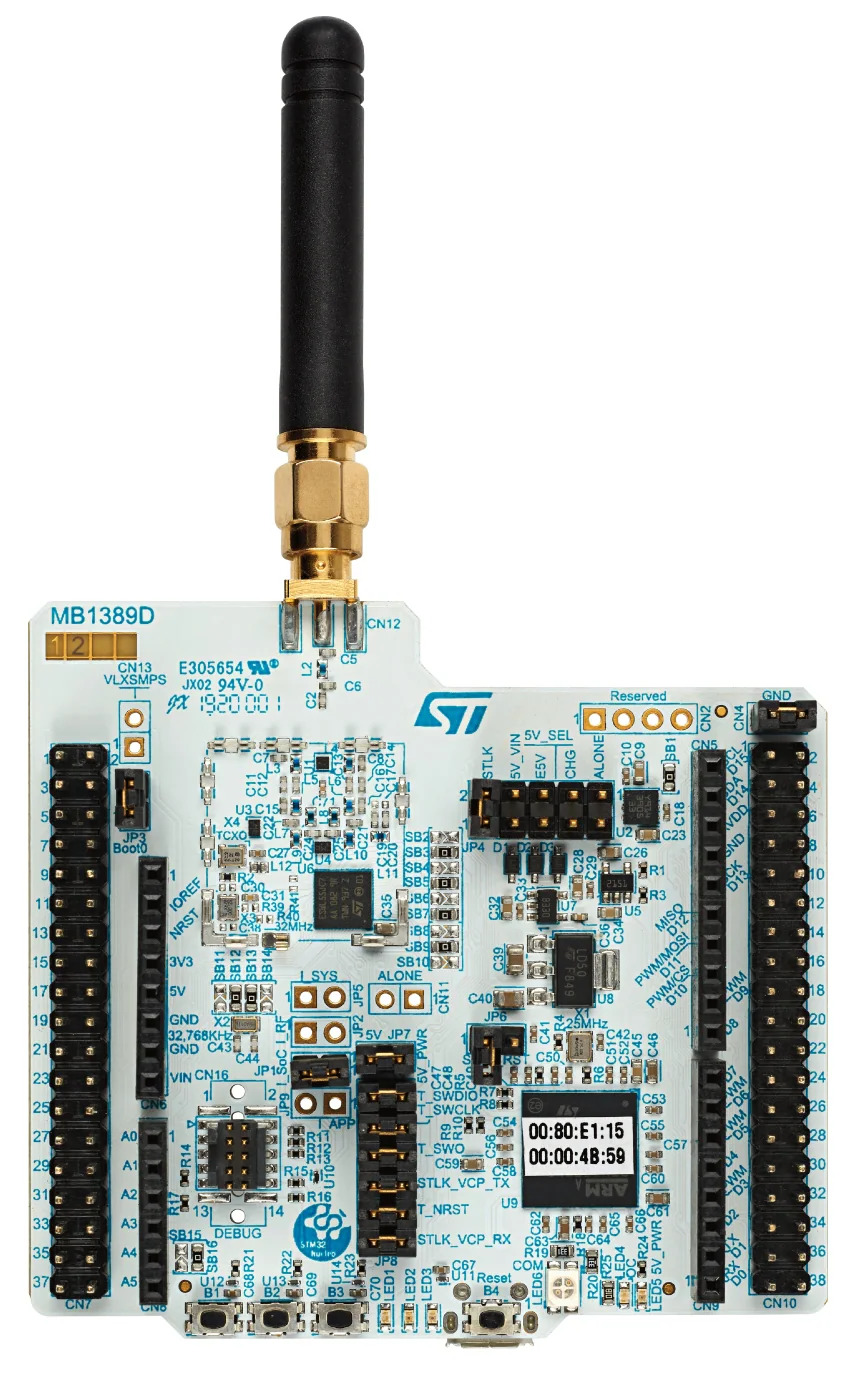
\includegraphics[width=.45\textwidth]{img/nucleo-wl55jc.jpg}}
    \subfloat[\label{fig:reference-design} STDES-WL5U4ILH]{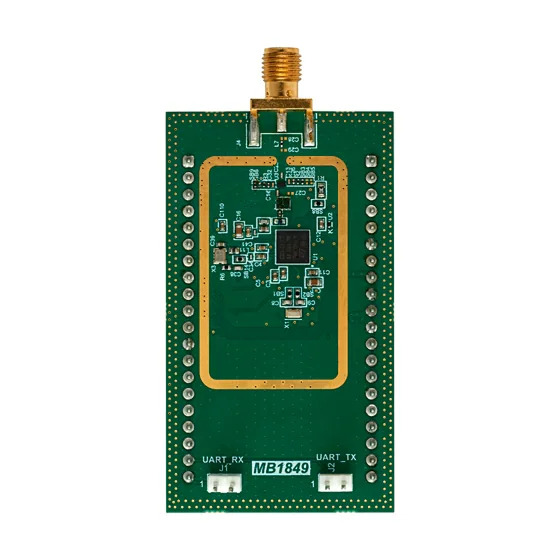
\includegraphics[width=.45\textwidth]{img/STDES-WL5U4ILH.jpg}}
    \caption{\label{fig:nucleo-and-reference} Nucleo development kit and the reference design board}
\end{figure}
%https://www.st.com/en/evaluation-tools/nucleo-wl55jc.html
%https://www.st.com/en/evaluation-tools/stdes-wl5u4ilh.html

Each of the designs focuses on optimizing different parameters depending on the application priorities and their codification follows table \ref{fig:reference-design-codification}, from which the defining features are apparent. For this work, application footprint was one of the top priorities, so the lower-power 15 dB version with IPD was selected.

IPD stands for Integrated Passive Device, it consists of a balun and a harmonic filter. This circuitry is usually realized using passive components, which is usually cheaper, but takes up more board space (see Figure \ref{fig:frontend-comparison}), is more prone to design mistakes and tuning mismatch. This particular IPD was specifically designed for STM32WL line of microcontrollers in this configuration.

\begin{figure}
    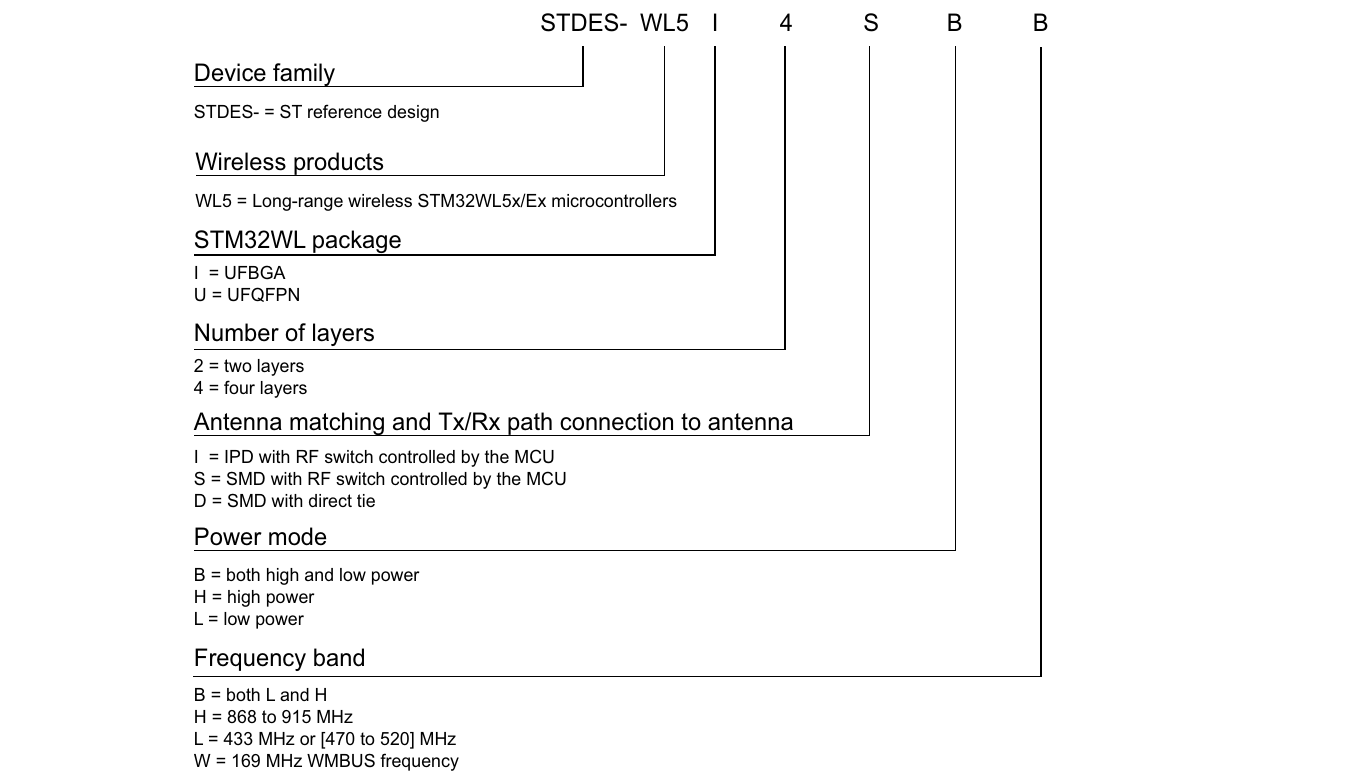
\includegraphics[width=\textwidth]{fig/STDES-xxxxxxx.png}
    \caption{\label{fig:reference-design-codification} STM32WL5x and STM32WLEx reference designs codification}
\end{figure}

\begin{figure}
    \centering
    \subfloat[discrete /wo RF switch (variant D)]{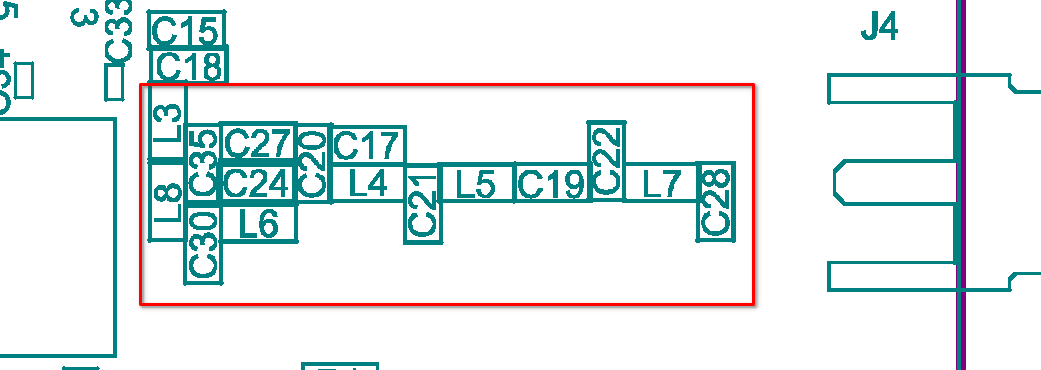
\includegraphics[width=.75\textwidth]{img/frontend-dlb.png}}\hfill
    \subfloat[discrete /w RF switch (variant S)]{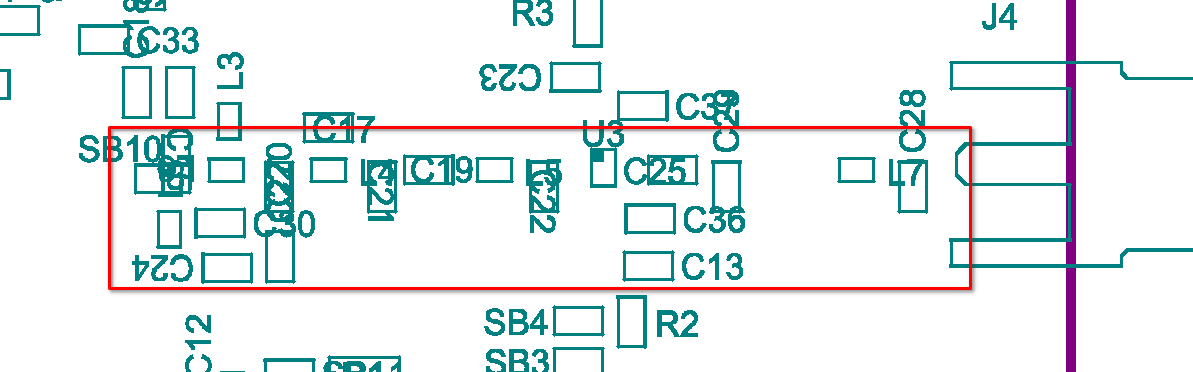
\includegraphics[width=.75\textwidth]{img/frontend-sbb.png}}\hfill
    \subfloat[IPD (variant I)]{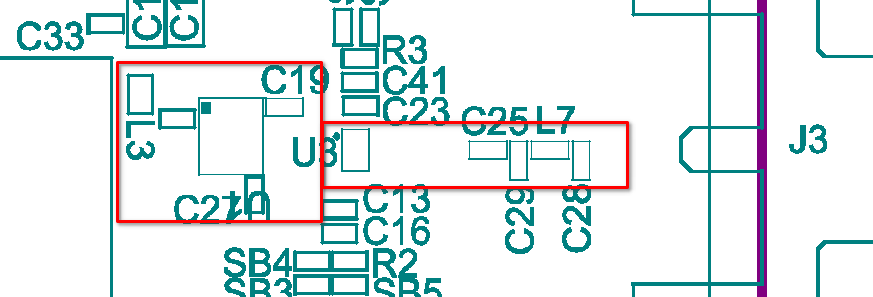
\includegraphics[width=.75\textwidth]{img/frontend-ilh.png}}
    \caption{\label{fig:frontend-comparison} Frontend layout and part selection comparison, components on the RF path highlighted. Reference designs selected for comparison were picked based on the similarity with the STDES-WL5U4ILH design.}
\end{figure}

One downside of using an IPD in this case is that it requires the use of an RF switch, because ST's IPDs are designed to work with separate receive and transmit paths. Again this is a tradeoff between complexity, cost and board space required. Fortunately only a Single Pole Double Throw switch is required, thus a simple switch such as the BGS12SN6 from Infineon is sufficient.

A 4 layer reference design was selected because it is anticipated it will allow a higher density layout, shrinking the module dimensions even further. UFQFPN package is preferred over UFBGA to stay compatible with lower cost manufacturing solutions. It is expected the design will use most of the available pins on the package, a complex fanout would be required if we were to go with the BGA variant, perhaps some space savings could be had at the cost of losing access to most of the pins, making any modifications to the design difficult to impossible, should the need arise.

In conclusion, the MCU choice is a culmination of tradeoffs where the prevention of mistakes, efficiency and familiarity were more important than the absolute performance and cost. This should not in any way hamper further improvements in succeeding versions of this hardware, while allowing the completion of Proof-of-Concept stages of this project. 

\subsection{Antenna}
Po dvou dnech hledání správné embedded antény jsem usoudil, že je to riskantní pokus a raději to nechám na příští revizi, protože je tam potřeba zvážit mnoho parametrů, což se teď dělá těžko - dám tam U.FL konektor pro externí anténu. Slibné varianty byly

\subsection{Power}
The selected MCU \ref{section:mcu} supports wide input voltage of 2-3.6 V thanks to its internal voltage regulation. It supports two modes - LDO, which does not require any additional external component at the cost of lower efficiency and the SMPS mode, utilizing a synchronous buck regulator, which is more efficient - this application will therefor attempt to implement the latter.

A separate, switchable power-rail is a feature deemed necessary by some considered applications in \ref{section:application-case-studies}. This can be achieved using a built-in MOSFET - such power rail could be used to save power even by powering off some parts of the module itself.

\subsection{Non-volatile memory}

\subsection{Conclusion}
We managed to meet all requirements set in \ref{section:final-requirements} except


\section{Sensor architecture}

Given the aim of this project

\subsection{Expected capacitance range}

\subsection{Measuring method}

\subsection{Battery and charging}
